\subsection{\Dc}
\begin{figure}[tb]
	\centering
	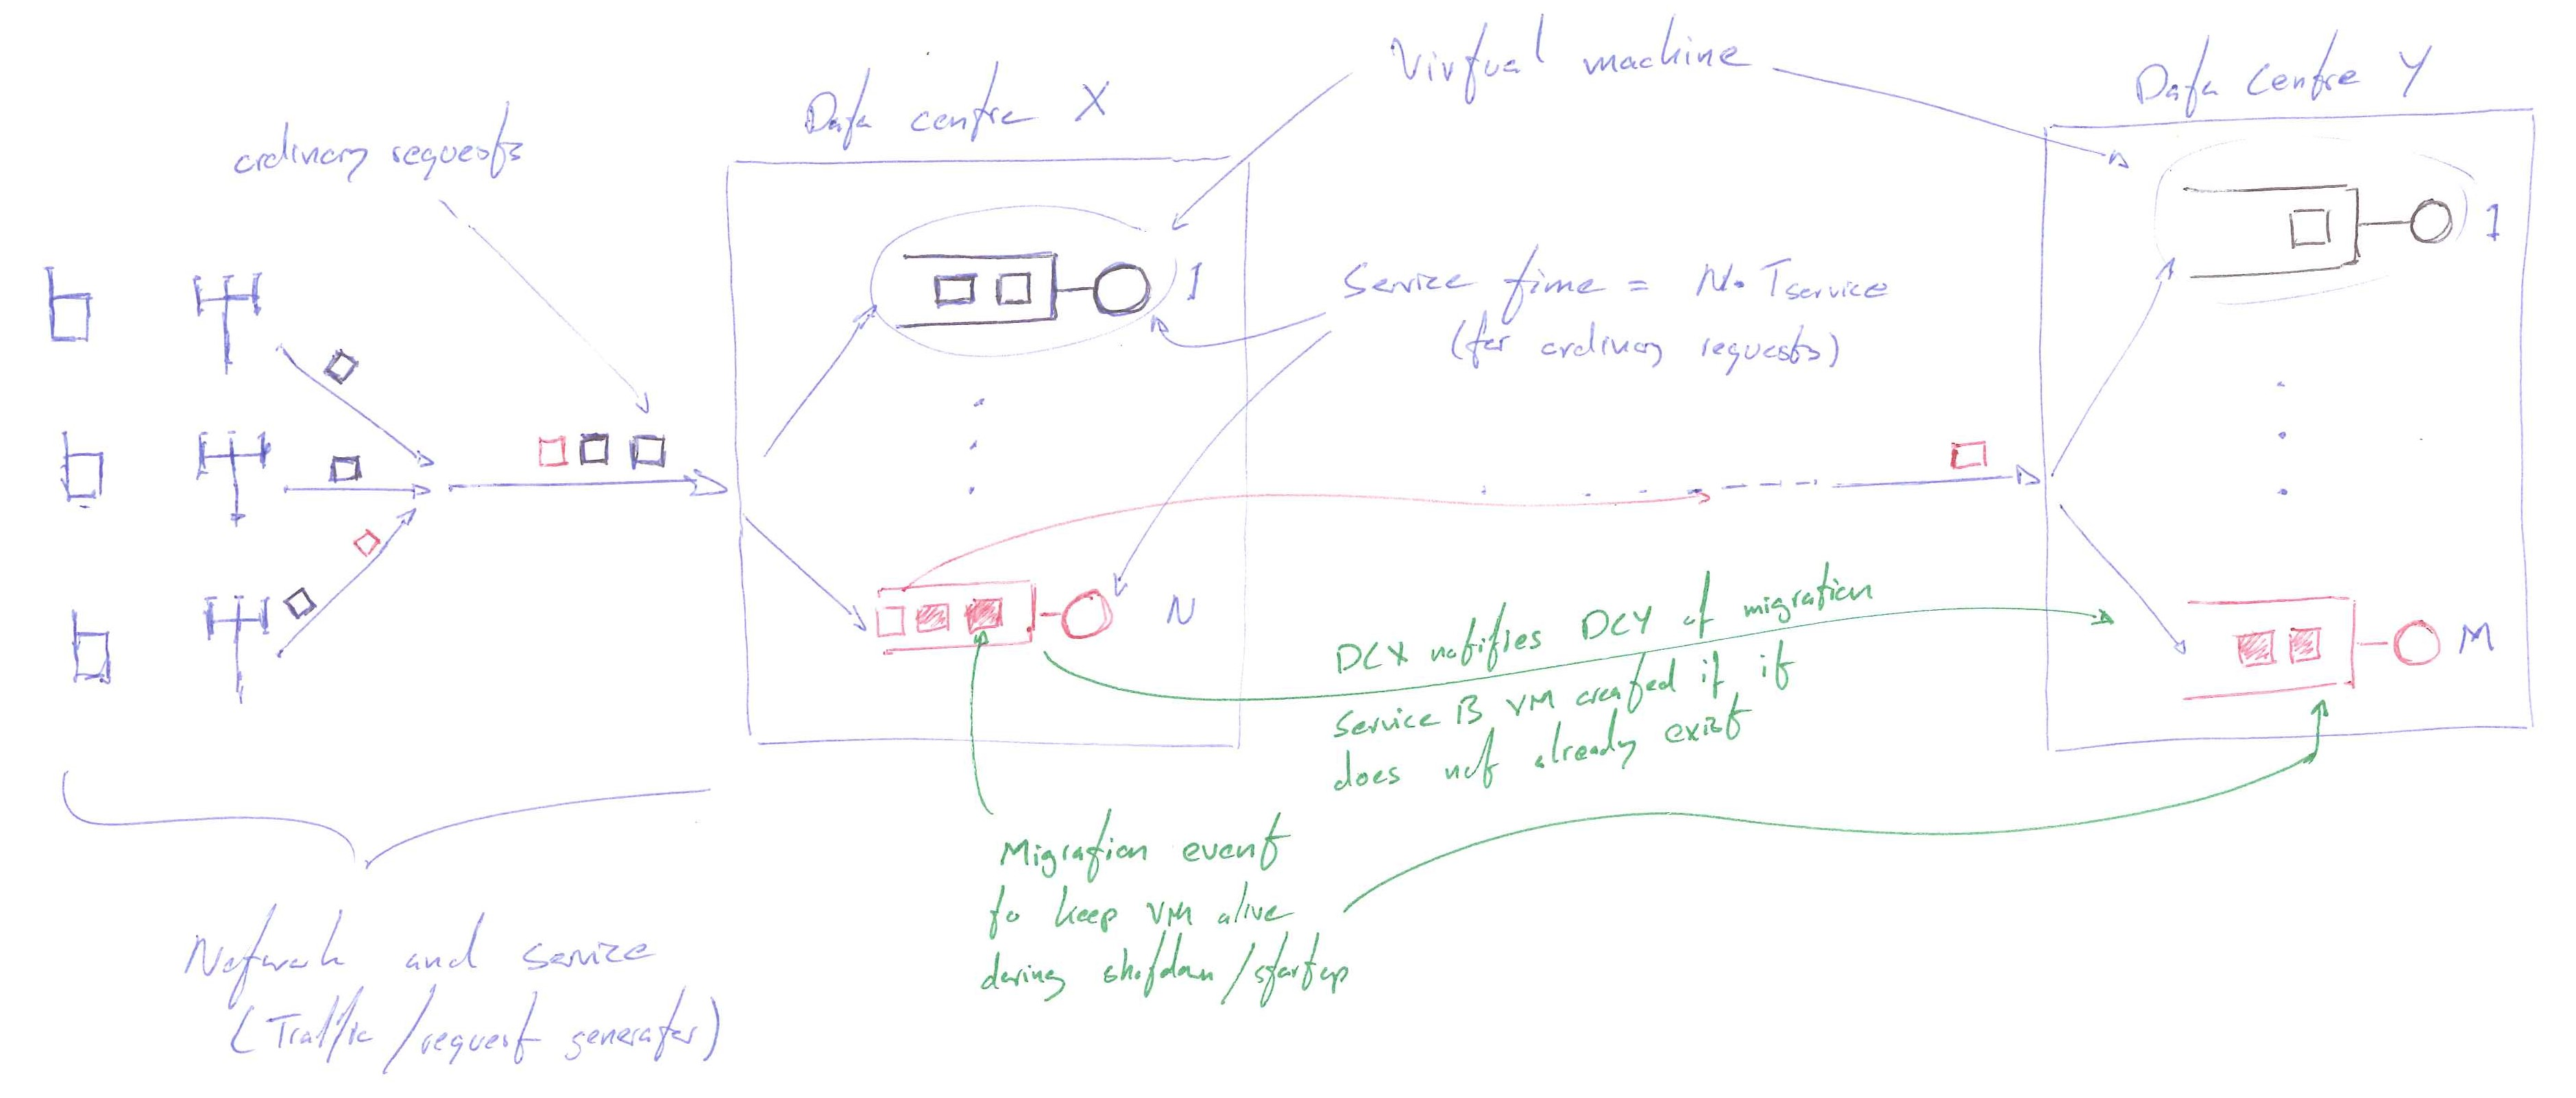
\includegraphics[width=\linewidth]{dc_model.jpg} 
	\caption{Performance model}
	\label{fig:performance_model}`
\end{figure}

To simplify the model of a \dc{} we will not consider CPU, memory, storage and intra \dc network separately.
Instead, in this paper, we will use an abstraction of one dimensional computational resource.

Hosting VMs in a \dc{} can be modeled in two ways: with or without competition for computational resource.

In the first approach, the resources of a \dc{} are aggregated in one pool that is continuously divisible.
%Each VM gets an equal part of available resources inversely proportional to the number of VMs hosted in the data center.
%The bigger is the number of VMs hosted in the \dc{}, the smaller amount of resources each of them gets.
The pool of resources is divided evenly among all VMs.
Hence, when the number of VMs hosted in the \dc{} increases, the amount of resources available for each VM shrinks.
Consequently the service time of processing requests of each VM lengthens.

In the second approach, the resources of a \dc{} are discrete and each computational unit is used exclusively by one VM.
Therefore, there is no influence of one VM on another.
To incorporate the fact that the amount of resources is finite we put a limit on the maximal number of VMs that can be hosted in one \dc{}.

\subsubsection{Overhead of VM Migration}
Migration has an influence on the service performance as well as on the resource availability on both source and destination \dc{}.
On the source side, apart from ordinary resource requirements due to serving requests, VM consumes resources for sending its image to the destination \dc{}.
In a case of postcopy live migration, VM at the source side still uses some resources even after the workload is redirected to the new location.
That is because the VM at destination side pulls remaining memory pages from the source \dc{}.

%The overhead of VM migration can be modeled in different ways depending on the manner how \dc resources are represented.

To model the overhead of migration on the service performance additional delay in the response time should be introduced.
Primarily, during the phase of transferring the image of VM, because of using a part of resources for I/O operations.
Additionally, in the case of the postcopy migration, delay occurs also for some time after redirecting the workload to the new \dc{}, due to the remote memory calls.

%That can be modeled by running two instances of VM during the time of migration, one per each DC.
When VMs compete for resources, running additional VM on the destination side introduces an overhead by increasing the response time of other collocated VMs.  

\subsubsection{Possible service hosting schemes}

\begin{itemize}
\item One service model, one VM is employed to host that service for each user.
\item One service model, each VM hosts multiple but each number of users, behaving as multiple services while still being compatible.
\end{itemize}


At all placement modes:
\begin{itemize}
\item Measure RTT for all packets at UE
\item Measure DC load
\item Measure ratio of requests generated vs. processed in \xcloud node
\item Identify the incurred VM migration load
\end{itemize}